\documentclass[11pt]{article}
\usepackage{url}
\usepackage{graphicx}
\usepackage{caption}
\usepackage{subcaption}
\usepackage{listings}
\usepackage{dsfont}
\usepackage{minted}


\usepackage{course}

\begin{document}

\ctitle{2}{Logistic Regression and Neural Networks}{
Nov. 15, 2022 at 11:59 pm
}
\author{}
\date{}
\vspace{-1in}
\maketitle
\vspace{-0.75in}

\blfootnote{Parts of this assignment are adapted from course material by Andrea Danyluk (Williams), Tom Mitchell, Matt Gormley and Maria-Florina Balcan (CMU), Stuart Russell (UC Berkeley), Carlos Guestrin (UW), Dan Roth (UPenn) and Jessica Wu (Harvey Mudd). }



\ifsoln 
\else
\section*{Submission instructions}
\begin{itemize}
\item 
Submit your solutions electronically on the course Gradescope site as PDF files.
\item Please package your code (.ipynb) for Problem 3 and submit it to BruinLearn.
\item If you plan to typeset your solutions, please use the LaTeX solution template. If you must submit scanned handwritten solutions, please use a black pen on blank white paper and a high-quality scanner app.
\end{itemize}
\fi

\ifnotsolution{\newpage}

\ifsoln 
\else
\clearpage
\fi

\section{Logistic Regression \problemworth{20}}

Consider the logistic regression model for binary classification that takes input features $\vect{x}_i\in R^m$ and predicts $y_i \in \{-1,1\}$. 
As we learned in class, the logistic regression model fits the probability $P(y_i = 1|\vect{x}_i)$ using the \textit{sigmoid} function:
\begin{equation}
    P(y_i = 1) = \sigma(\vect{w}^T \vect{x}_i+b) = \frac{1}{1+ \exp(-\vect{w}^T\vect{x}_i-b)},
\end{equation}
where the sigmoid function is as follows, for any $z\in\mathbb{R}$,
\[
\sigma(z)=(1+\exp(-z))^{-1}.
\]
Given $N$ training data points, we learn the logistic regression model by minimizing the following loss function:
\begin{equation}
\label{eq:j}
J(\vect{w}, b) = 
  \frac{1}{N} \sum_{i=1}^{N}\log\Big(1+\exp\big(-y_i(\vect{w}^T \vect{x}_i+b)\big)\Big).
\end{equation}
\begin{enumerate}
\item \itemworth{7} Prove the following. For any $z\in\mathbb{R}$, the derivative of the sigmoid function is as follows: 
\begin{equation*}
    \frac{d\sigma(z)}{dz} = \sigma(z)\big(1 - \sigma(z)\big).
\end{equation*}
(Hint: use the chain rule. And $\frac{d}{dx}\exp(x)=\exp(x)$.)

\solution{

\begin{gather*}
  \sigma = (1 + exp(-z))^{-1} \\
  \begin{split}
    \frac{d\sigma}{dz} & = -exp(-z)(1+exp(-z))^{-2} = \frac{-exp(-z)}{(1+exp(-z))^2}  \\
    & = \left( \frac{-1}{1 + exp(-z)}\right) \left(\frac{-exp(z)}{1+exp(-z)}\right)\\
    & = -\sigma(z)\left(\frac{-1-exp(z) + 1}{1+exp(-z)}\right) \\
    & = \sigma(z)(1 - \frac{1}{1+exp(-z)}) = \sigma(z)(1 - \sigma(z))
  \end{split}
\end{gather*}
$\hfill \Box$
}
\end{enumerate}

Suppose we are updating the weight $\mathbf{w}$ and bias term $b$ with the gradient descent algorithm and the learning rate is $\alpha$. We can derive the update rule as
\[w_j \leftarrow w_j - \alpha\frac{\partial J(\mathbf{w},b)}{\partial w_j},\; \text{where}\; \frac{\partial J(\mathbf{w},b)}{\partial w_j}=\frac{1}{N}\sum_{i=1}^N  \Big(\sigma\big(y_i(\vect{w}^T \vect{x}_i+b)\big) - 1\Big) y_ix_{i,j}\]
where $w_j$ denotes the j-th element of the weight vector $\mathbf{w}$ and $x_{i,j}$ denotes the j-th element of the vector $\mathbf{x}_i$. And 
\[
b\leftarrow b-\alpha\frac{\partial J(\mathbf{w},b)}{\partial b},\; \text{where} \;\frac{\partial J(\mathbf{w},b)}{\partial b}=\frac{1}{N}\sum_{n=1}^N\Big(\sigma\big(y_i(\vect{w}^T \vect{x}_i+b)\big) - 1\Big) y_i
\]

We now compare the stochastic gradient descent algorithm for logistic regression with the Perceptron algorithm. Let us define residue for example $i$ as $\delta_i=1-\sigma\big(y_i(\vect{w}^T \vect{x}_i+b)\big)$. Assume the learning rate for both algorithms is $\alpha$.

\begin{enumerate}
\setcounter{enumi}{1}
\item \itemworth{5} If the data point $(\mathbf{x}_i,y_i)$ is correctly classified with high confidence, say $y_i=1$ and $\mathbf{w}^\top\mathbf{x}_i + b = 5$. What will be the residue? For the logistic regression, what will be the update with respect to this data point? What about the update of the Perceptron algorithm? (\textbf{Hint}: you may assume $\sigma(5)\approx 0.9933$. The answer should take the form $w_j\leftarrow w_j-[?]$ or $w_j\leftarrow w_j+[?]$ where you fill in $[?]$. You can directly use $x_{i,j}$ and $\alpha$ as variables.)

\solution{
  $\delta_i = 1 - \sigma(5) \approx .0067$ 

  Logistic Regression: $w_j \leftarrow w_j - \alpha(-.0067x_{i,j})$ \\
  Perceptron: Not updated since there was no mistake.
}

\item \itemworth{5} If the data point $(\mathbf{x}_i,y_i)$ is misclassified, say $y_i=1$ and $\mathbf{w}^\top\mathbf{x}_i + b = -1$. What will be the residue and how is the weight updated for the two algorithms? (\textbf{Hint}: you may assume $\sigma(-1)\approx 0.2689$.)

\solution{
  $\delta_i = 1 - \sigma(-1) \approx .7311$ 

  Logistic Regression: $w_j \leftarrow w_j - \alpha(-.7311x_{i,j})$ \\
  Perceptron: $w \leftarrow w + \alpha x_i$
}

\item \itemworth{3} For the update step in SGD and perceptron algorithm, is the influence of the input data $\mathbf{x}_i$ of the same magnitude? If not, what is the difference?

\solution{
  Influence larger for perceptron since the whole weight vector is updated rather than just the jth element.
}


\end{enumerate}

\section{Regularization \problemworth{10}}
Data is separable in one dimension if there exists a threshold $t$ such that all data that have values less than $t$ in this dimension have the same class label. Suppose we train logistic regression for infinite iterations according to our current gradient descent update on the training data that is separable in at least one dimension.
\begin{enumerate}
\item \itemworth{2} (multiple choice) If the data is linearly separable in dimension $j$, i.e. $x_{i,j}<t$ for all $(\mathbf{x}_i,y_i)$ such that $y_i=-1$. Which of the following is true about the corresponding weight $w_j$ when we train the model for infinite iterations?

\begin{itemize}
\item[(A)] The weight $w_j$ will be 0.
\item[(B)] The weight $w_j$ will be encouraged to grow continuously during each iteration of SGD
and can go to infinity or -infinity.
\end{itemize}

\solution{
  B is true.
}

\item \itemworth{5} We now add a new term (called $l2$-regularization) to the loss function
\begin{equation}
\label{eq:j}
J(\vect{w}, b) = 
  \frac{1}{N} \sum_{i=1}^{N}\log\Big(1+\exp\big(-y_i(\vect{w}^T \vect{x}_i+b)\big)\Big) +  0.1 \sum^M_{j=0}w_j^2.
\end{equation}
What will be the update rule of $w_j$ for the new loss function?

\solution{
  \[
    w_j \leftarrow w_j - \alpha \left[ \frac{1}{N}\sum_{i=1}^N  \Big(\sigma\big(y_i(\vect{w}^T \vect{x}_i+b)\big) - 1\Big) y_ix_{i,j} + 0.2 \sum_{j = 0}^M w_j \right]
  \] 
}

\item \itemworth{3} How does $l2$ regularization help correct the problem in (a)?

\solution {
  The problem occurs because the model tries to predict as close to 0 or 1 as possible, but it can never reach 0 or 1 due to the way the loss function is defined. So the weights are pushed infinitely in the respective direction to make this happen. By adding the weight as a term outside of the sigmoid, we prevent the weight from increasing to infinity to get as close to 0 or 1 as possible since increasing infinitely would take the whole term to infinity rather than the target.

  \href{https://stats.stackexchange.com/questions/469799/why-is-logistic-regression-particularly-prone-to-overfitting-in-high-dimensions}{Here} is a good source explaining this in more detail.
}

\end{enumerate}
\section{Neural Networks and Deep Learning \problemworth{20}}

In the following set of questions, we will discuss feed-forward and backpropagation for neural networks.

We will consider two kinds of hidden nodes/units for our neural network. The first cell (Cell A) operates as a weighted sum with no activation function. Given a set of input nodes and their weights, it outputs the weighted sum. The second cell (Cell B) operates as a power function. It takes only one input along with the weight and outputs the power of input to the weight as the output. We provide illustrations for both the nodes in Figure~\ref{fig:nn-nodes}. Note that $\mathbf{x} = [x_1, x_2, \dots, x_n]^T$ and $\mathbf{w} = [w_1, w_2, \dots, w_n]^T$.

\begin{figure}[h]
\centering
\begin{subfigure}{.5\textwidth}
  \centering
  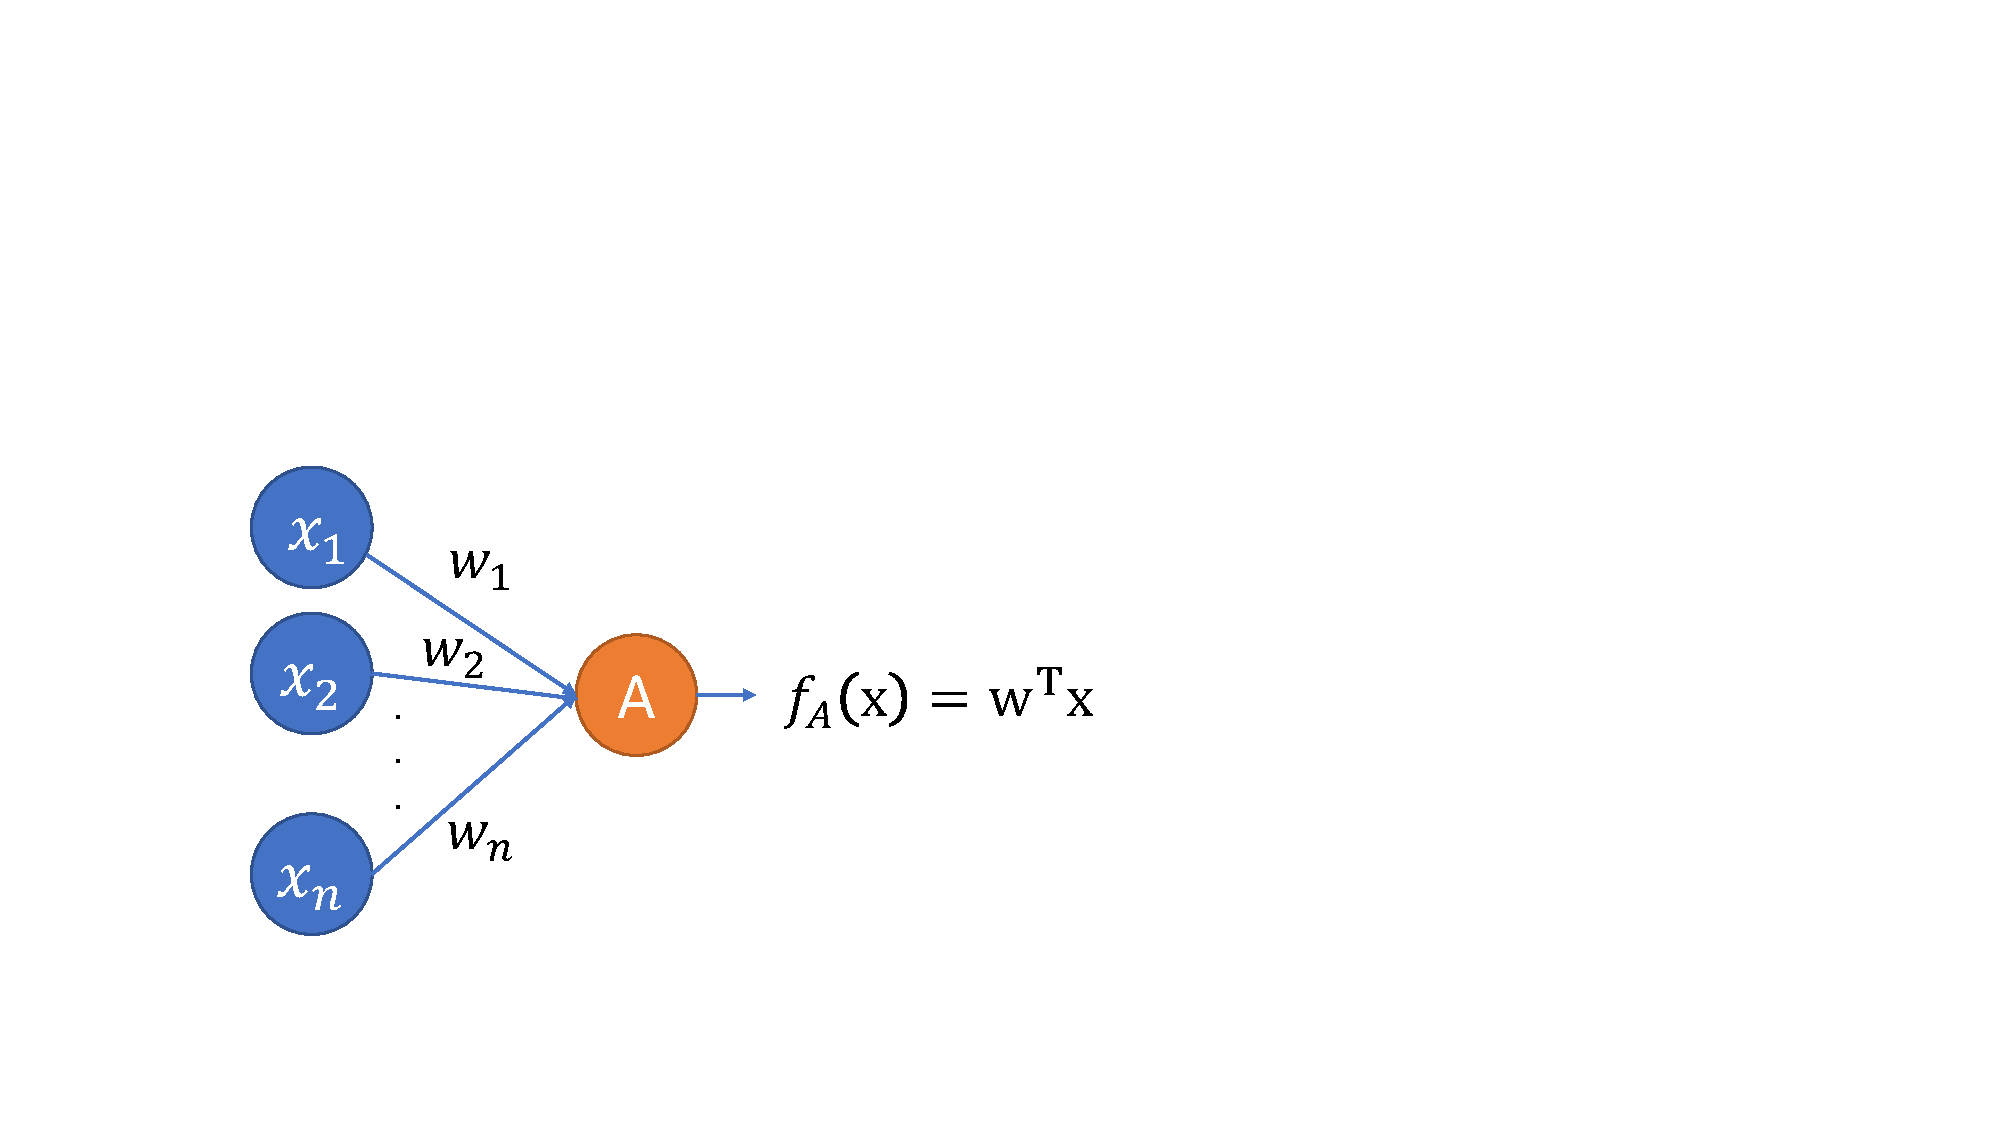
\includegraphics[width=.8\linewidth]{hw2-images/cell-a.pdf}
  \caption{}
  \label{fig:sub1}
\end{subfigure}%
\begin{subfigure}{.5\textwidth}
  \centering
  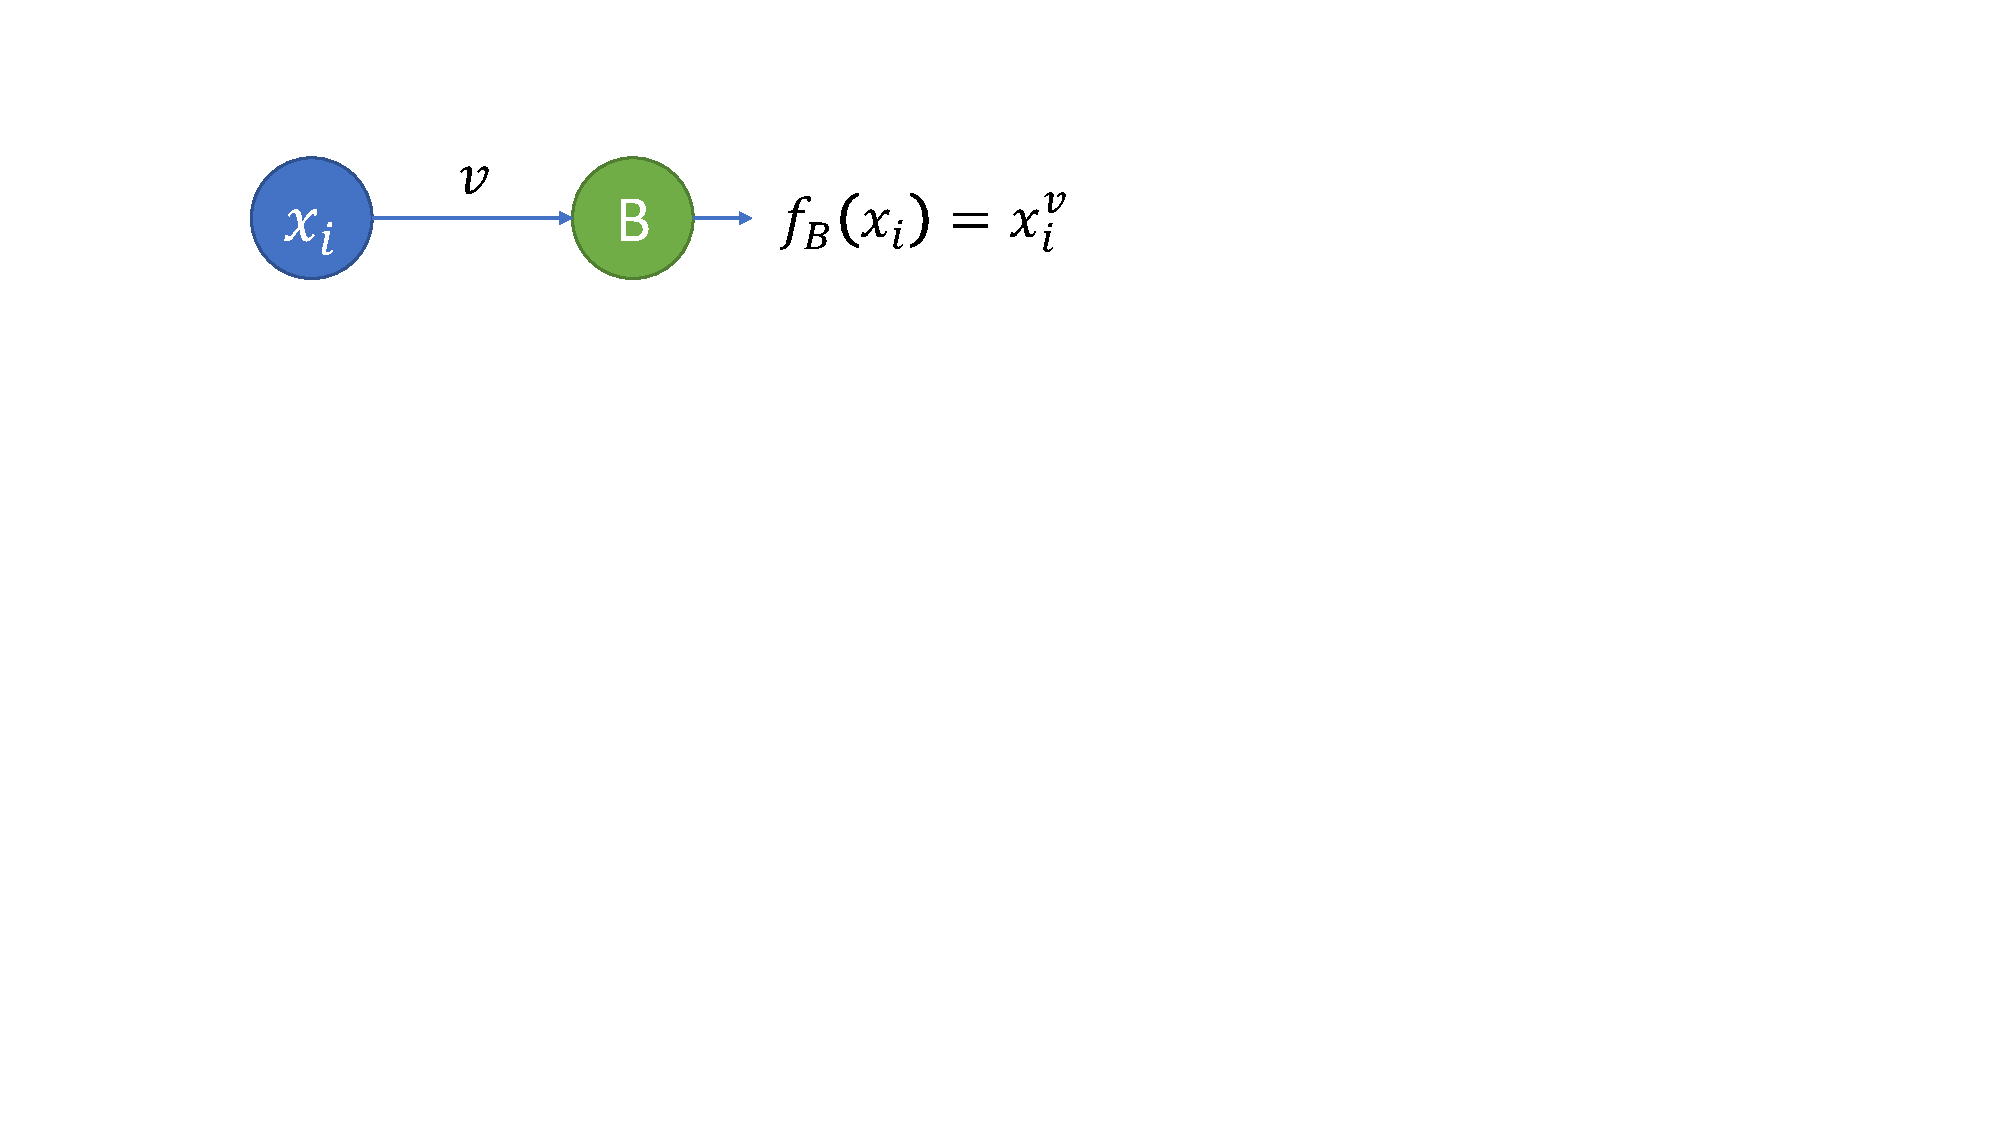
\includegraphics[width=.8\linewidth]{hw2-images/cell-b.pdf}
  \caption{}
  \label{fig:sub2}
\end{subfigure}
\caption{An illustration of Cell A and Cell B used in the neural network. (a) On the left, we have Cell A - Weighted sum. It simply computes the weighted sum over the input nodes. (b) On the right, we have Cell B - It computes power of the input node over the weight}
\label{fig:nn-nodes}
\end{figure}

Using these two kinds of hidden nodes, we build a two-layer neural network as shown in Figure~\ref{fig:nn-network}. The inputs to the neural network is $\mathbf{x} = [x_1, x_2, x_3]^T$ and the output is $\hat{y}$. The parameters of the model are $\mathbf{v} = [v_1, v_2, v_3]^T$ and $\mathbf{w} = [w_1, w_2, w_3]^T$.

\begin{figure}[h]
    \centering
    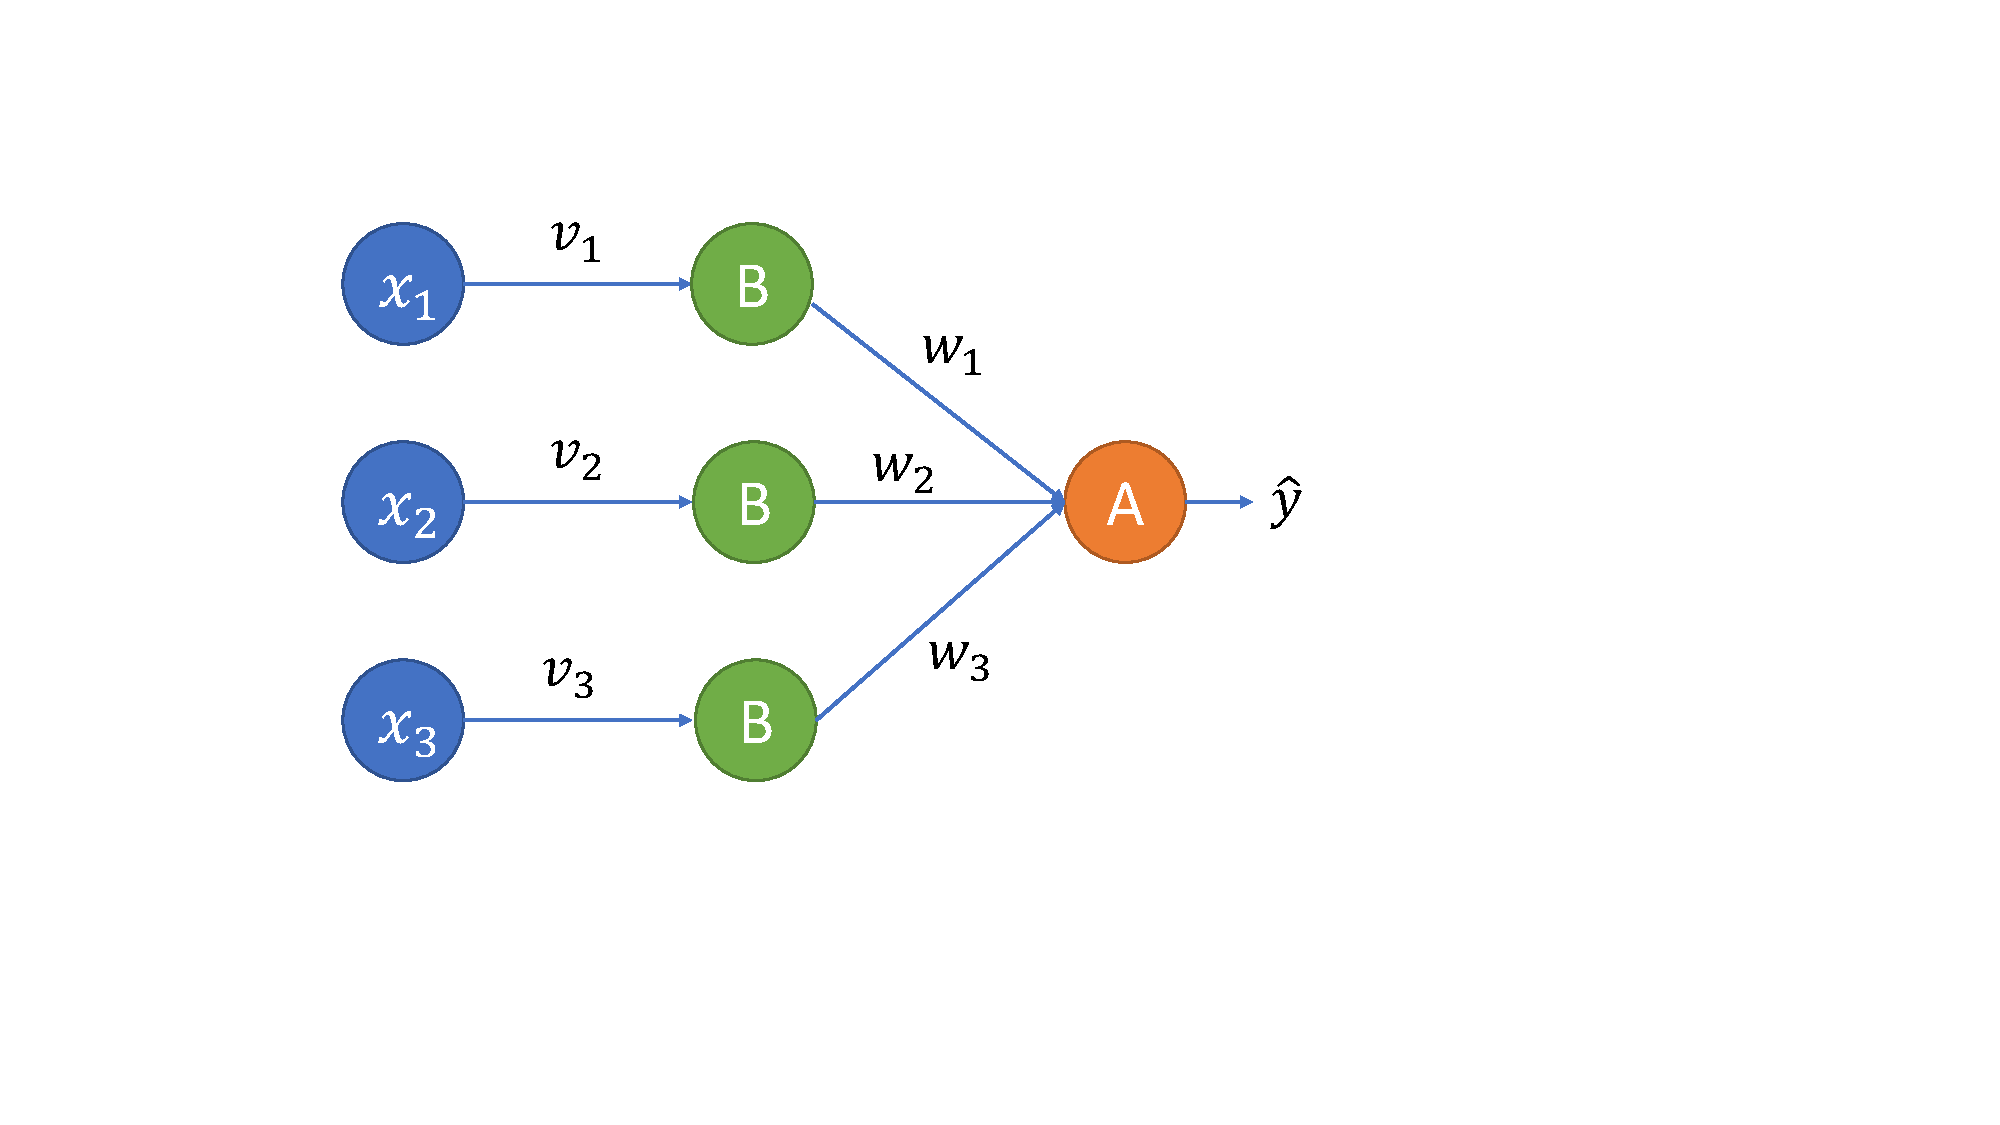
\includegraphics[width=.5\linewidth]{hw2-images/neural-network.pdf}
    \caption{Architecture of the neural network.}
    \label{fig:nn-network}
\end{figure}

\begin{enumerate}
    \item \itemworth{4}
    We would like to compute the feed-forward for the network. Mathematically, compute the expression for $\hat{y}$ given the neural network in terms of $\mathbf{x}, \mathbf{v}, \mathbf{w}$.
    
    
    
    \item \itemworth{2}
    Utilizing the expression for $\hat{y}$ computed in (a), compute the predicted value $\hat{y}$ when $\mathbf{x} = [1,3,2]^T, \mathbf{v}=[1,0,2]^T, \mathbf{w}=[-4,3,1]^T$
    
    
\end{enumerate}

We want to now utilize the backpropagation algorithm to update the weights of this neural network. First we will compute the gradients with respect to the weights. For the following parts, we are only interested in updating $v_1$ and $w_1$ in the network.

\begin{enumerate}
    \setcounter{enumi}{2}
    \item \itemworth{5} Let's derive the expression for gradients for the weights. More specifically, compute the expressions for $\frac{\partial \hat{y}}{\partial w_1}$ and $\frac{\partial \hat{y}}{\partial v_1}$. Using the values described in part (b), compute the final values of these expressions. (\textbf{Hint:} Use the expression computed in part (a))
    
    
    
    \item \itemworth{3} Assuming the loss function is $\mathcal{L} = (y - \hat{y})^2$ where $y$ is the true value of the output and $\hat{y}$ is the predicted output from the neural network. Compute the expression for  $\frac{\partial \mathcal{L}}{\partial \hat{y}}$. Let the actual value of $y = 5$. What will the value for this expression be?
    
    
    
    \item \itemworth{3} Using parts (c) and (d), compute the values for the expressions for $\frac{\partial \mathcal{L}}{\partial v_1}$ and $\frac{\partial \mathcal{L}}{\partial w_1}$. (\textbf{Hint:} Use the chain rule)
    
    
\end{enumerate}

We will finally use the gradient descent algorithm to update the weights for $v_1$ and $w_1$. Note that the gradient descent update formula for a parameter $w$ is given as $w \leftarrow w - \eta \frac{\partial \mathcal{L}}{\partial w}$. Assume the learning rate $\eta = 1$ for the following question.

\begin{enumerate}
    \setcounter{enumi}{5}
    \item \itemworth{3} Using the gradient descent update rule explained above, compute the updated values for $v_1$ and $w_1$.
    
    
\end{enumerate}
\newpage
\section{Programming exercise : Applying decision trees and k-nearest neighbors \problemworth{55}}

\section*{Introduction}

\begin{figure}[ht]
\centering
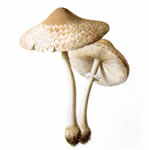
\includegraphics[scale=2.5]{mushroom.jpg}
\end{figure}

In this problem, we will work on a mushroom classification task. The dataset is adapted from the \href{https://archive.ics.uci.edu/ml/datasets/mushroom}{UCI Machine Learning Repository} and it contains descriptions of hypothetical samples corresponding to 23 species of gilled mushrooms. Each mushroom is described in terms of physical characteristics, and the goal is to classify mushrooms as \emph{edible} or \emph{poisonous}. We will apply decision trees and k-nearest neighbors. Since this dataset is relatively simple for classification, we only use 6 features out of 22 features in the original dataset. Features we use include: 
cap-shape, cap-color, gill-color, stalk-root, veil-type, ring-number.


For all the coding, please refer to the following Colab notebook  
\href{https://colab.research.google.com/drive/13_JuaV8-uwTBO7YEheYGm3cjl8DZB8HA?usp=sharing}{Fall2022-CM146-HW1.ipynb}. 

\textbf{Before executing or writing down any code, please make a copy of the notebook and save it to your own google drive by clicking the “File” $\rightarrow$ “Save a copy in Drive”.} 

\begin{figure}[ht]
\centering
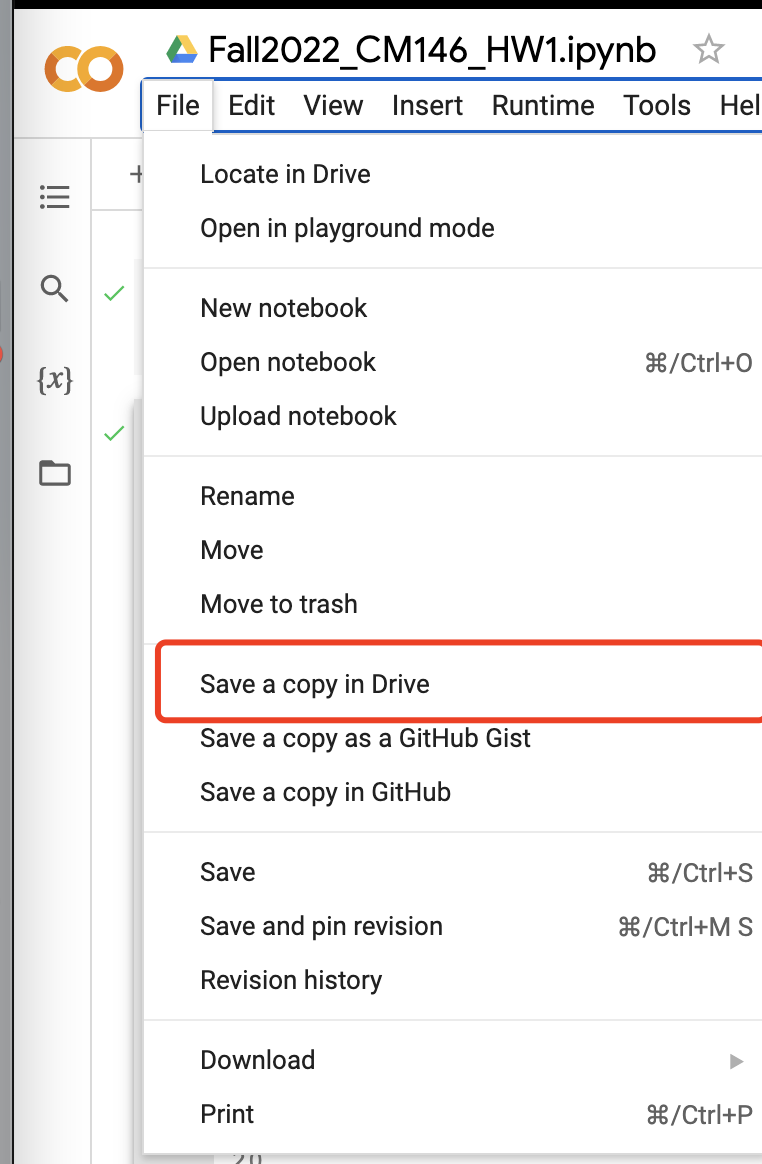
\includegraphics[scale=0.25]{save-colab-to-drive.png}
\end{figure}

You will probably be prompted to log into your Google account. Please make sure all the work you implement is done on your own saved copy. You won’t to able to make changes on the the original notebook shared with the entire class.

The notebook has marked blocks where you need to code:
\begin{verbatim}
### ========== TODO : START ========== ###
### ========== TODO : END ========== ###
\end{verbatim}

\section*{Submission instructions for programming problems}
\begin{itemize}
\item Please save the execution output in your notebook. When submitting, please export the notebook to a \verb|.ipynb| file by clicking ``File'' $\rightarrow$ ``Download .ipynb'' and upload the notebook to BruinLearn.

\item
Your code should be commented appropriately. Importantly:
\begin{itemize}[nosep]
\item Your name should be at the top of the file.
\item Each class and method should have an appropriate doctsring.
\item Include some comments for anything complicated.
\end{itemize}

There are many possible solutions to this assignment, which makes coding style and comments important for graders to conveniently understand the code. 

\item Please submit all the plots and the rest of the solutions (other than codes) to Gradescope.
\end{itemize}


\subsection{Visualizing Features \problemworth{5}}
One of the first things to do before trying any formal machine learning technique is to dive into the data. This can include looking for funny values in the data, looking for outliers, looking at the range of feature values, what features seem important, etc.
We have already included the code for loading the data, converting all the categorical features to numerical one.

Make histograms for each feature, separating the examples by class (i.e., edible or poisonous).
This should produce 6 plots, one for each feature, and each plot should have two overlapping histograms, with the color of the histogram indicating the class. 
The code has been included in \texttt{plot\_histograms} and \texttt{plot\_histogram} functions, and you do not need to code by yourself.

For each feature, what trends do you observe in the data? (Please only describe the general trend. No need for more than two sentences per feature.) 

\solution{
    \begin{itemize}
        \item cap-shape: For both edible and inedible mushrooms the distribution is apprximately symmetrical with edible being slightly skewed left and inedible being slightly skewed right.
        \item cap-color: For both, cap color seems to be evenly spread throughout all possible cap colors. There is no clear trend.
        \item gill-color: For inedible, most gill-color is $<$ 4 while there is no clear trend for edible.
        \item stalk-root: Inedible is largely skewed right while there is no clear trend for edible.
        \item veil-type: There is a clear split between edible and inedible; edible is veil-type $>$ 0 while inedible is veil-type $<$ 0.
        \item ring-number: There is a split between edible and inedible; edible is (mostly) ring-number $>$ 1 while inedible is (mostly) ring-number $<$ 1.
    \end{itemize}
}

\subsection{Training and Evaluating Models \problemworth{55}}

Now, let's use \verb|scikit-learn| to train a \verb|DecisionTreeClassifier| and \verb|KNeighborsClassifier| on the data.
Using the predictive capabilities of the \verb|scikit-learn| package can be carried out in three steps: initializing the model, fitting it to the training data, and predicting new values.

\begin{enumerate}

\item \itemworth{5} Before trying out any classifier, it is often useful to establish a \emph{baseline}. We have implemented one simple baseline classifier, \verb|MajorityVoteClassifier|, that always predicts the majority class from the training set. Read through the \verb|MajorityVoteClassifier| and its usage and make sure you understand how it works.

Your goal is to implement and evaluate another baseline classifier, \verb|RandomClassifier|, that predicts a target class according to the distribution of classes in the training data set. For example, if 85\% of the examples in the training set have \verb|edible = 0| and 15\% have \verb|edible = 1|, then, when applied to a test set, \verb|RandomClassifier| should randomly predict 85\% of the examples as \verb|edible = 0| and 15\% as \verb|edible = 1|.

Implement the missing portions of \verb|RandomClassifier| according to the provided specifications. Then train your \verb|RandomClassifier| on the entire training data set, and evaluate its training error. 

\solution{
    Error: 0.503
}


\item \itemworth{5} Now that we have a baseline, train and evaluate a \verb|DecisionTreeClassifier| (using the class from \verb|scikit-learn| and referring to the documentation as needed). Make sure you initialize your classifier with the appropriate parameters; in particular, use the `entropy' criterion discussed in class. What is the training error of this classifier?

\solution{
    Error: 0.055
}

\item \itemworth{10} Similar to the previous question, train and evaluate a \verb|KNeighborsClassifier| (using the class from \verb|scikit-learn| and referring to the documentation as needed). Use $k$=3, 11 and 19 as the number of neighbors and report the training error of this classifier. If we implement KNN model from scratch, what operations we should do in the \verb|fit| method?

\solution{
    Error (k = 3): 0.064
    Error (k = 11): 0.070
    Error (k = 19): 0.076

    If implemented from scratch, we would need to store the data in our chosen data structure within the fit method. 
}

\item \itemworth{10} So far, we have looked only at training error, but as we learned in class, training error is a poor metric for evaluating classifiers. Let's use cross-validation instead.

Implement the missing portions of \verb|error(...)| according to the provided specifications. You may find it helpful to use \verb|StratifiedShuffleSplit(...)| from \verb|scikit-learn|. To ensure that we always get the same splits across different runs (and thus can compare the classifier results), set the \verb|random_state| parameter to be the same (e.g., 0).


Next, use your \verb|error(...)| function to evaluate the training error and (cross-validation) test error and test micro averaged \href{https://scikit-learn.org/stable/modules/generated/sklearn.metrics.f1_score.html?highlight=f1\%20score#sklearn.metrics.f1_score}{F1 Score} of each of your four models (for the \verb|KNeighborsClassifier|, use $k=11$). To do this, generate a random $85/15$ split of the training data, train each model on the $85\%$ fraction, evaluate the error on both the $85\%$ and the $15\%$ fraction, and repeat this $100$ times to get an average result.


\item \itemworth{10} One way to find out the best value of $k$ for \verb|KNeighborsClassifier| is $n$-fold cross validation.
Find out the best value of $k$ using 5-fold cross validation and the F1 Score metric. Run cross validation for all odd numbers ranging from 1 to 100 as the number of neighbors.

Then plot the validation score against the number of neighbors, $k$. Include this plot in your writeup. What is the best value of $k$ and what is the corresponding score?

You may find the \verb|cross_val_score(...)| from \verb|scikit-learn| helpful. 

\solution{
    The best value of k is 13 with a score of 0.9297682709447415.

    \begin{center}
        \img{./3e.png}
    \end{center}
}


\item \itemworth{10} One problem with decision trees is that they can \emph{overfit} to training data, yielding complex classifiers that do not generalize well to new data. Let's see whether this is the case.

One way to prevent decision trees from overfitting is to limit their depth. Run 20-fold cross-validation for increasing depth limits $1,2,\ldots,20$. 

Then plot the average training F1 Score and test F1 score against the depth limit. Include this plot in your writeup, making sure to label all axes and include a legend for your classifiers. What is the best depth limit to use for this data? Do you see overfitting? Justify your answers using the plot.

You may find \verb|cross_validate| from \verb|scikit-learn| helpful when you want both training scores and validation scores.

\end{enumerate}


\end{document}